% ============================================================
% Contenido de demostración (idéntico en las tres variantes)
% Modelo Lotka--Volterra: matemáticas, figura, código, citas.
% ============================================================

\section{Modelos depredador--presa}

El modelo de Lotka--Volterra describe la interacción entre una población de
presas $x(t)$ y una de depredadores $y(t)$~\cite{volterra1926,murray2002}:
\begin{align}
  \frac{dx}{dt} &= \alpha\, x - \beta\, x y, \label{eq:lv-x}\\[2pt]
  \frac{dy}{dt} &= -\gamma\, y + \delta\, x y, \label{eq:lv-y}
\end{align}
donde $\alpha$ es la tasa de crecimiento de las presas, $\gamma$ la tasa de
mortandad de los depredadores, y $\beta$, $\delta$ cuantifican el encuentro
entre ambas especies.

\begin{definition}[Equilibrio de coexistencia]
El sistema~\eqref{eq:lv-x}--\eqref{eq:lv-y} admite, además del
equilibrio trivial $(0,0)$, el punto de coexistencia
$(x^{*}, y^{*}) = \left(\tfrac{\gamma}{\delta},\, \tfrac{\alpha}{\beta}\right)$.
\end{definition}

\begin{theorem}[Estabilidad del equilibrio de coexistencia]
\label{thm:lv}
Para $\alpha, \beta, \gamma, \delta > 0$, la matriz jacobiana del sistema
evaluada en $(x^{*}, y^{*})$ tiene autovalores puramente imaginarios
$\lambda_{\pm} = \pm i \sqrt{\alpha \gamma}$; el equilibrio es un centro
(linealmente neutro) y las trayectorias cercanas son órbitas cerradas.
\end{theorem}

\begin{proof}
El jacobiano es
$J(x,y) = \begin{pmatrix} \alpha - \beta y & -\beta x \\ \delta y & -\gamma + \delta x \end{pmatrix}$,
de modo que $J(x^{*}, y^{*}) = \begin{pmatrix} 0 & -\beta\gamma/\delta \\ \delta\alpha/\beta & 0 \end{pmatrix}$,
con $\operatorname{tr} J = 0$ y $\det J = \alpha\gamma > 0$.
La \cref{fig:phase} muestra el retrato de fases para
$\alpha = \beta = \gamma = \delta = 1$.
\end{proof}

\begin{figure}[htbp]
  \centering
  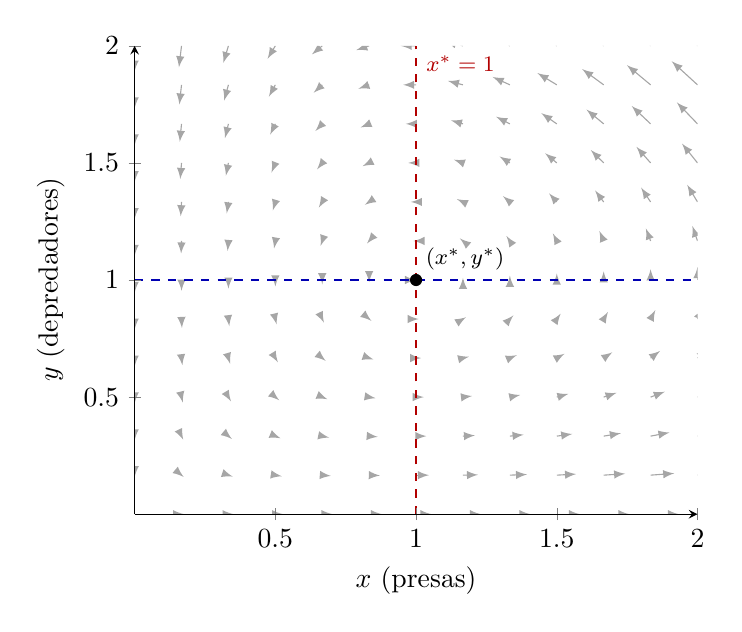
\begin{tikzpicture}
    \begin{axis}[
        view={0}{90}, domain=0:2, y domain=0:2,
        xmin=0, xmax=2, ymin=0, ymax=2,
        samples=13, width=0.72\linewidth,
        xlabel={$x$ (presas)}, ylabel={$y$ (depredadores)},
        axis lines=middle, grid=both, grid style={gray!15},
        xlabel near ticks, ylabel near ticks,
      ]
      \addplot3[gray!70, -latex, quiver={
          u={x - x*y}, v={-y + x*y}, scale arrows=0.055}] (x,y,0);
      \draw[red!70!black, thick, dashed] (axis cs:1,0) -- (axis cs:1,2)
        node[below right, font=\footnotesize]{$x^{*}=1$};
      \draw[blue!70!black, thick, dashed] (axis cs:0,1) -- (axis cs:2,1)
        node[above right, font=\footnotesize]{$y^{*}=1$};
      \fill (axis cs:1,1) circle (2.2pt) node[above right, font=\footnotesize]{$(x^{*},y^{*})$};
    \end{axis}
  \end{tikzpicture}
  \caption{Retrato de fases del modelo de Lotka--Volterra con
  $\alpha=\beta=\gamma=\delta=1$. Las nulas roja y azul son los
  \emph{nullclines}; el equilibrio $(1,1)$ es un centro.}
  \label{fig:phase}
\end{figure}

\aside{Los autovalores imaginarios puros no prueban estabilidad: el
sistema conservativo tiene un primer integral $V(x,y)=\delta x - \gamma
\ln x + \beta y - \alpha \ln y$, y sus curvas de nivel son las órbitas
cerradas~\cite{strogatz2015}.}

\subsection{Integración numérica en Python}

La \cref{eq:lv-x}--\eqref{eq:lv-y} se integra con Euler explícito:

\begin{minted}[fontsize=\small, framesep=4pt, frame=lines]{python}
import numpy as np

alpha, beta, gamma, delta = 1.0, 1.0, 1.0, 1.0

def lv(u, t):
    """Campo vectorial de Lotka-Volterra."""
    x, y = u
    return np.array([alpha*x - beta*x*y,
                     -gamma*y + delta*x*y])

dt, T = 0.01, 20.0        # paso temporal y horizonte
u = np.array([1.2, 0.6])  # condición inicial
for t in np.arange(0, T, dt):
    u = u + dt * lv(u, t)
print(f"estado final: x = {u[0]:.3f}, y = {u[1]:.3f}")
\end{minted}

\subsection{Simulación con agentes en NetLogo}

La misma dinámica puede explorarse como un modelo basado en
agentes~\cite{netlogo}, donde cada presa y depredador es una tortuga:

\begin{minted}[fontsize=\small, framesep=4pt, frame=lines]{lexer/netlogo.py:NetLogoLexer}
globals [presas-iniciales depredadores-iniciales]
turtles-own [energia]

to setup
  clear-all
  create-turtles presas-iniciales [
    setxy random-xcor random-ycor
    set color green  set energia 10
  ]
  create-turtles depredadores-iniciales [
    setxy random-xcor random-ycor
    set color red
  ]
  reset-ticks
end

to go
  ask turtles [
    ifelse color = red
      [ let presa min-one-of turtles with [color = green]
                        [distance-to self]
        if presa != nobody [ face presa  fd 1.2 ] ]
      [ fd 1  set energia energia - 1
        if energia < 2 [ die ] ]
  ]
  tick
end
\end{minted}

\subsection{Dinámica discreta: del mapa logístico al caos}

Al discretizar el crecimiento logístico con tiempo
discreto~\cite{may1976} aparece el mapa
\begin{equation}
  N_{t+1} = r\, N_t \left(1 - \frac{N_t}{K}\right),
  \label{eq:logistic-map}
\end{equation}
que, bajo el cambio $z_t = N_t/K$, se reduce al mapa logístico
$z_{t+1} = \mu\, z_t (1 - z_t)$ con $\mu = 1 + r$. Para $\mu > 3{,}57$
la dinámica es caótica: un modelo determinista de una sola variable
produce trayectorias impredecibles, un fenómeno que May argumentó que
debe tomarse en serio en la gestión de poblaciones reales.

% ---------------------------------------------------------
\nocite{edelstein2007,tongqft}
\printbibliography[heading=bibintoc, title={Referencias}]
